\documentclass[8pt]{beamer}

\setbeamertemplate{background canvas}[vertical shading][bottom=cyan!10,top=blue!10]

\usetheme{Warsaw}
\usefonttheme[onlysmall]{structurebold}

% pour le fichiers .pdf
\usepackage{graphicx}
\usepackage{color}
% pour les fichiers .png
% \usepackage{pgf,pgfarrows}
% \usepackage{pgf,pgfarrows}
\usepackage{amsmath,amssymb}
\usepackage{textcomp}
\usepackage{Math_Notations}
\usepackage{multitoc}
\usepackage{mdwtab}
\setbeamercovered{dynamic}
\DeclareMathOperator*{\argmin}{argmin}

\title[OpenTURNS Developer Training]{OpenTURNS Developer Training: the platform overview}
\author[OpenTURNS Consortium, 2019]
{
  Trainer : R\'egis LEBRUN \\
  Airbus \\
  regis.lebrun@airbus.com
}

\date[March 22-25th 2011]
{
  Developers training \\

  \begin{center}
    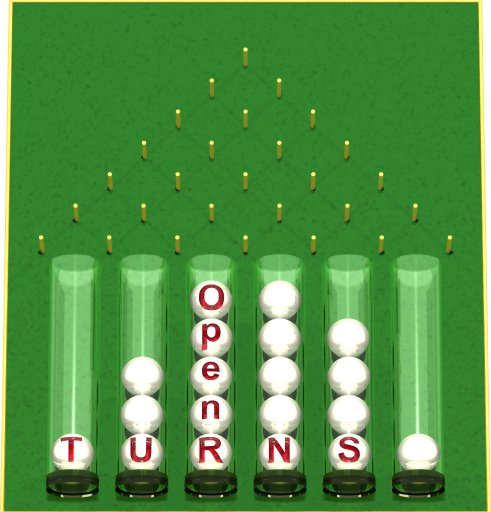
\includegraphics[height=2cm]{logoOT.jpg}
  \end{center}
}

\subject{OpenTURNS Developers Training}

% \part<presentation>{Corps de presentation}


\begin{document}

\frame{\titlepage}

% necessaire pour la table des matieres
\part{Main part}

% table des matieres
\begin{frame}
  \Large
  \frametitle{Platform overview}
  \tableofcontents[part=1]
\end{frame}
%%%%%%%%%%%%%%%%%%%%%%%%% 
% The OpenTURNS package %
%%%%%%%%%%%%%%%%%%%%%%%%% 
\section[The story]{The story}
%%%%%%%%%%%%%%%% 
% Introduction %
%%%%%%%%%%%%%%%% 
\begin{frame}
  \frametitle{Introduction}
  \begin{block}{Objectives}
    The objectives of this course is to give a broad overview of the OpenTURNS project and the resulting platform. We will cover the following points:
    \begin{itemize}
    \item The history of the project,
    \item The global organization of the platform,
    \item The multi-layer view of the library,
    \item The several usages of the platform.
    \end{itemize}
  \end{block}
\end{frame}
%%%%%%%%%%% 
% History %
%%%%%%%%%%% 
\begin{frame}
  \frametitle{History}
  \begin{block}{2005-2011: 7 years of partnership}
    \begin{itemize}
    \item[2005] Conception, setup of the compilation infrastructure, setup of the development environment, first base classes.
    \item[2006] main development of the C++ library
    \item[2007] python binding. First release the 10th of May (release 0.9.0). Web site. 6 additional releases (0.9.1, 0.9.2, 0.10.0, 0.11.0, 0.11.1, 0.11.2).
    \item[2008] 4 releases (0.11.3, 0.12.0, 0.12.1, 0.12.2, 0.12.3). Main new features: more distributions, more wrapping facilities.
    \item[2009] 2 releases (0.13.0, 0.13.1). Main new features: multithreaded wrappers, new algorithms, polynomial chaos expansion.
    \item[2010] 1 release (0.13.2). First windows port. Modularization of the python binding. Better integration of the data model with python native structures. Work on the parallelization of the algorithms. First work on stochastic processes and random fields.
    \item[2011] Sparse chaos implementation. Coming soon: first development of stocahstic processes.
    \end{itemize}
  \end{block}
\end{frame}
\section[The platform]{The platform}
%%%%%%%%%%%%%%%%%% 
% Global picture %
%%%%%%%%%%%%%%%%%% 
\begin{frame}
  \frametitle{The platform at a glance, developer's view}
  \centering \resizebox{!}{8cm}{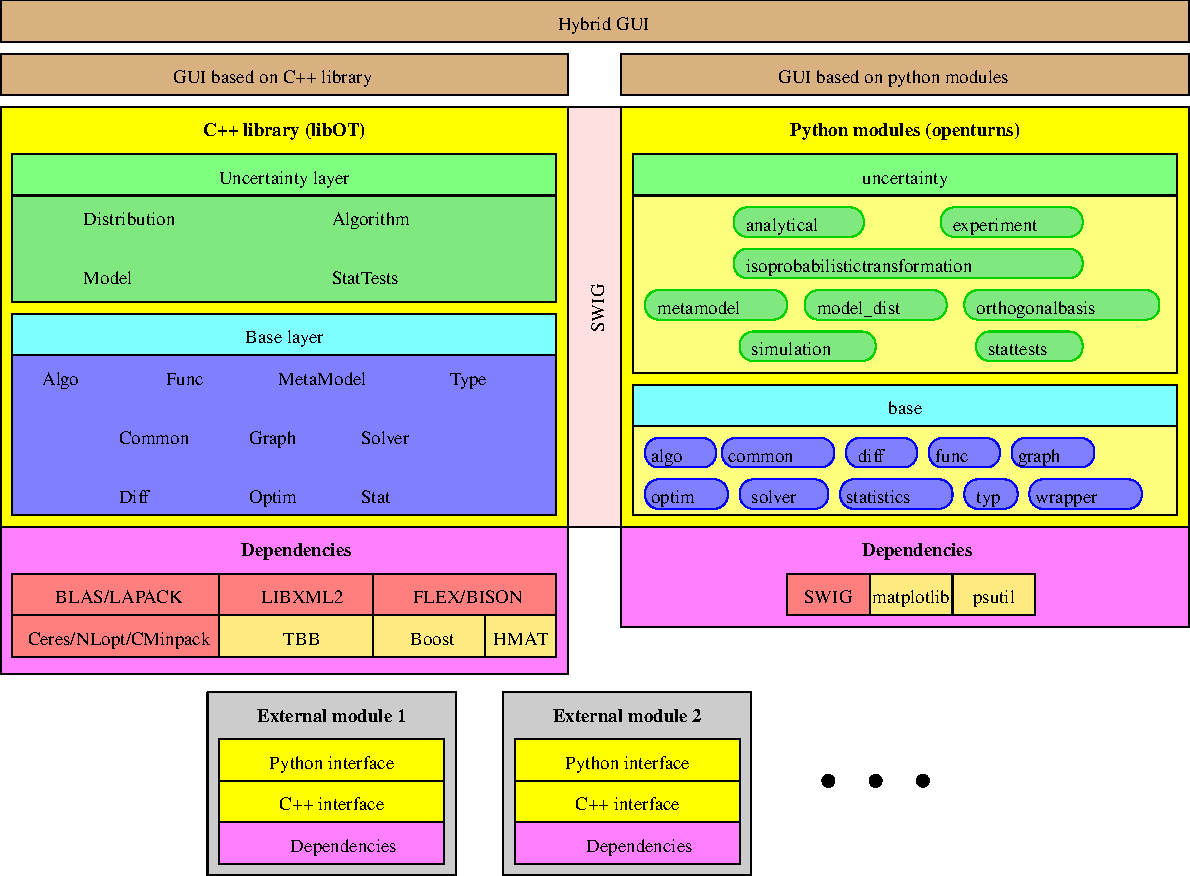
\includegraphics{GlobalPicture.pdf}}
\end{frame}
\begin{frame}
  \frametitle{The platform at a glance, developer's view}
  \begin{block}{The big parts}
    \begin{itemize}
    \item The \alert{core} of the OpenTURNS platform is a \alert{C++ library}, made of about 500 classes of various size. The library has a multi-layered architecture that is materialized by both the namespace hierarchy and the source tree.
    \item The \alert{main user interface} is the \alert{python module}, automatically generated from the C++ library using the wrapping software SWIG. It allows for a usage of OptnTURNS through python scripts of any level of complexity.
    \item The library relies on relatively \alert{few dependencies} and most of them are optional.
    \item A service of \alert{modules} is provided in order to extend the capabilities of the platform from the outside.
    \item Several \alert{GUIs} have already been built on top of the C++ library or the Python module.
    \end{itemize}
  \end{block}
\end{frame}
%%%%%%%%%%%%%%%%%%% 
% The C++ library %
%%%%%%%%%%%%%%%%%%% 
\begin{frame}
  \frametitle{The C++ library}
  \begin{block}{A multilayered library}
    The two main layers in the C++ library are the \alert{Base} layer and the \alert{Uncertainty} layer.
    \begin{itemize}
    \item \alert{Base} layer: it contains all the classes not related to the probabilistic concepts. It covers the elementary data types (vectors as NumericalPoint, samples as NumericalSamples), the concept of models (NumericalMathFunction), the linear algebra (Matrix, Tensor) and the general interest classes (memory management, resource management);
    \item \alert{Uncertainty} layer: it contains all the classes that deal with probabilistic concepts. It covers the probabilistic modelling (Distribution, RandomVector), the stochastic algorithms (MonteCarlo, FORM), the statistical estimation (DistributionFactory), the statistical testing (FittingTest)
    \end{itemize}
    A class in the Uncertainty layer can use any class in the Base or the Uncertainty layer. A class in the Base layer can ONLY USE classes in the Base layer.
  \end{block}
\end{frame}
\begin{frame}
  \frametitle{The C++ library}
  \begin{block}{A monolythic library?}
    The C++ library is provided as a unique object file (libOT.so) created using the libtool technology. As such, it is a monolythic library (of about 8Mo stripped), but internally it is made of numerous sub-libraries, one for each folder in the source tree. A future objective is to modularize this library in order to spped-up both the compilation time and the loading time.
  \end{block}
  \begin{block}{A parallel library}
    Some of the most time-consuming algorithms have been parallelized using the Thread Building Block technology (INTEL), a C++ library that allows for a parallelization of C++ code in a shared memory model. One of the objectives of OpenTURNS is the ability to execute external simulation softwares on large simulation models for a large amount of independent data sets. As such, OpenTURNS provides basic functionalities to distribute the executions of these simulations on a multiprocessors(cores) infrastructure using the low-level pthread technology or the TBBs.
  \end{block}
\end{frame}
%%%%%%%%%%%%%%%%%%%%% 
% The python module %
%%%%%%%%%%%%%%%%%%%%% 
\begin{frame}
  \frametitle{The python module}
  \begin{block}{Interfacing python and C++ libraries: SWIG}
    In order to provide a convenient interface to the user, the C++ library can be manipulated as a set of Python modules (18) that are organized through a hierarchy, on top of which stands the openturns module. The binding of the library is done almost automatically by SWIG (Simplified Wrapper Interface Generator) through a set of SWIG interface files.\\
    An additional significant work has been made in order to ease the interation between the OpenTURNS objects and the native Python objects.\\
    A unique feature of the Python interface is the ability to wrap a Python function into an OpenTURNS concept of mathematical function, namely the NumericalMathFunction, using a specific class: the OpenTURNSPythonFunction. Using this mechanism, it is possible to adress virtually all the scenarios of coupling with an external simulation software.
  \end{block}
\end{frame}
%%%%%%%%%% 
% The OS %
%%%%%%%%%% 
\begin{frame}
  \frametitle{The target OSes}
  \begin{block}{A linux platform that works on windows}
    The historic platform of OpenTURNS is linux. The first stage of developments have been made on 32 bits Intel Linux platforms (debian, mandriva), then the (minor) adaptations have been made in order to run on 64 bits Intel platforms as well.\\
    Currently, the platform works on the following platforms:
    \begin{itemize}
      \item Debian 32 bits / 64 bits (Hetch to current);
      \item Mandriva 32 bits / 64 bits (2005 to current);
      \item Windows 32 bits / 64 bits (XP, Vista, seven).
    \end{itemize}
    The development platform remains Linux, the Windows version is obtain by cross compilation under Linux (using the mingw tools). A native Windows version is planed.
  \end{block}
\end{frame}
%%%%%%%%%%%%%%%%%%%%%%%%%%%%%%%%%% 
% The development infrastructure %
%%%%%%%%%%%%%%%%%%%%%%%%%%%%%%%%%% 
\section[The development infrastructure]{The development infrastructure}
\begin{frame}
  \frametitle{The development infrastructure}
  \begin{block}{Compilation infrastructure}
    Two alternative compilation infrastructures are present: the historic one (autotools + libtools) and the newcommer (CMake). For now, only the first infrastructure is running smoothly. It covers:
    \begin{itemize}
    \item The detection and configuration aspects of the platform;
    \item The dependency management of the sources;
    \item The generation of parallel makefiles;
    \item The regression tests;
    \item The library packaging.
    \end{itemize}
    The use of the autotools also greatly simplify the Linux packaging (.deb, .rpm). The CMake infrastructure is still in a beta state, but should greatly improve the configuration and compilation steps, and provide a way to compile the Windows version using Microsoft compilers, in order to easily reuse the C++ library in native Windows projects.
  \end{block}
\end{frame}
\begin{frame}
  \frametitle{The development infrastructure}
  \begin{block}{Versioning system}
    The versioning system used for the development of the whole platform is Subversion (SVN), on top of which stands a TRAC website.
    \begin{itemize}
    \item \alert{Apache Subversion} is a software versioning and a revision control system issued from the Apache project. It is used for both the sources of the platform and the documentation, as well as for the development of modules.
    \item \alert{Trac} is an open source, web-based project management and bug-tracking tool. Trac allows hyperlinking information between a bug database, revision control and wiki content. It also serves as a web interface to several revision control systems including Subversion.
    \end{itemize}
  \end{block}
  \begin{block}{Repositories}
    Three repositories are used for the development of the platform, its documentation and its modules. This choice has been made for the following reasons:
    \begin{itemize}
    \item The time scale is not the same for these three activities;
    \item The teams are different partly in term of people, but mainly in term of expertise.
    \end{itemize}
  \end{block}
\end{frame}
%%%%%%%%%%%%%%%%%%%%%%%%%%%%%%%%%% 
% The development infrastructure %
%%%%%%%%%%%%%%%%%%%%%%%%%%%%%%%%%% 
\begin{frame}
  \frametitle{The development infrastructure}
  \begin{block}{Platform repository}
    This repository is in charge of both the C++ library source code and the python interface. It has the following organization, which is quite standard:
    \begin{itemize}
    \item A trunk that stores the source code of the upcoming version of the platform. The rule is to have only source code that pass with success all the tests embedded with both the library and the python module.
    \item Several development branches, dedicated to contributors or to specific developments. There are curently 6 active branches.
    \item A branch for the tags with one entry for each release candidate or official releases. 17 releases have been tagged so far.
    \end{itemize}
    The usage of this infrastructure is described in the Contribution Guide, one of the several documents that come with the platform. In particular, a specific role is assigned to an \alert{integrator}, in charge of the merges from the different branches into the trunk.
  \end{block}
\end{frame}
%%%%%%%%%%%%%%%%%%%%%%%%%%%%%%%%%% 
% The development infrastructure %
%%%%%%%%%%%%%%%%%%%%%%%%%%%%%%%%%% 
\begin{frame}
  \frametitle{The development infrastructure}
  \begin{block}{Documentation repository}
    This repository is in charge of the whole documentation of the platform (10 different documents). It has been separated from the main repository by the middle of 2009 in order to allow for more frequent updates of the documentation with respect to the whole platform. It shares the same structure as the main repository:
    \begin{itemize}
    \item A trunk that stores the source code of the upcoming version of the documentation. The rule is to have only LaTeX source code able to generate the PDF version of all the documents.
    \item Several documentation branches, dedicated to contributors. There are currently 3 active branches.
    \item A branch for the tags with one entry for each release of the documentation. 4 releases have been tagged since july 2009.
    \end{itemize}
    The usage of this infrastructure is the same as for the main repository.
  \end{block}
\end{frame}
%%%%%%%%%%%%%%%%%%%%%%%%%%%%%%%%%% 
% The development infrastructure %
%%%%%%%%%%%%%%%%%%%%%%%%%%%%%%%%%% 
\begin{frame}
  \frametitle{The development infrastructure}
  \begin{block}{Modules repository}
    This repository is dedicated to the development of extra functionalities that have not yet been integrated into the main library, due to the lack of maturity of their dependencies for example. This repository is organized in a different way than the previous repositories:
    \begin{itemize}
    \item There is a branch for each module
    \item Within these branches, \alert{the same organization as the main repository is proposed} but the developers are free to organize the things the way they want. Nevertheless, the commitment to the standard organization should ease the future integration into the mainstream development.
    \item For now, there are 2 active modules and one template.
    \end{itemize}
  \end{block}
\end{frame}
%%%%%%%%%%%%%%%%%%%%%%%%%%%%%%%%%% 
% The development infrastructure %
%%%%%%%%%%%%%%%%%%%%%%%%%%%%%%%%%% 
\begin{frame}
  \frametitle{Trac interface: the timeline}
  \centering \resizebox{!}{7cm}{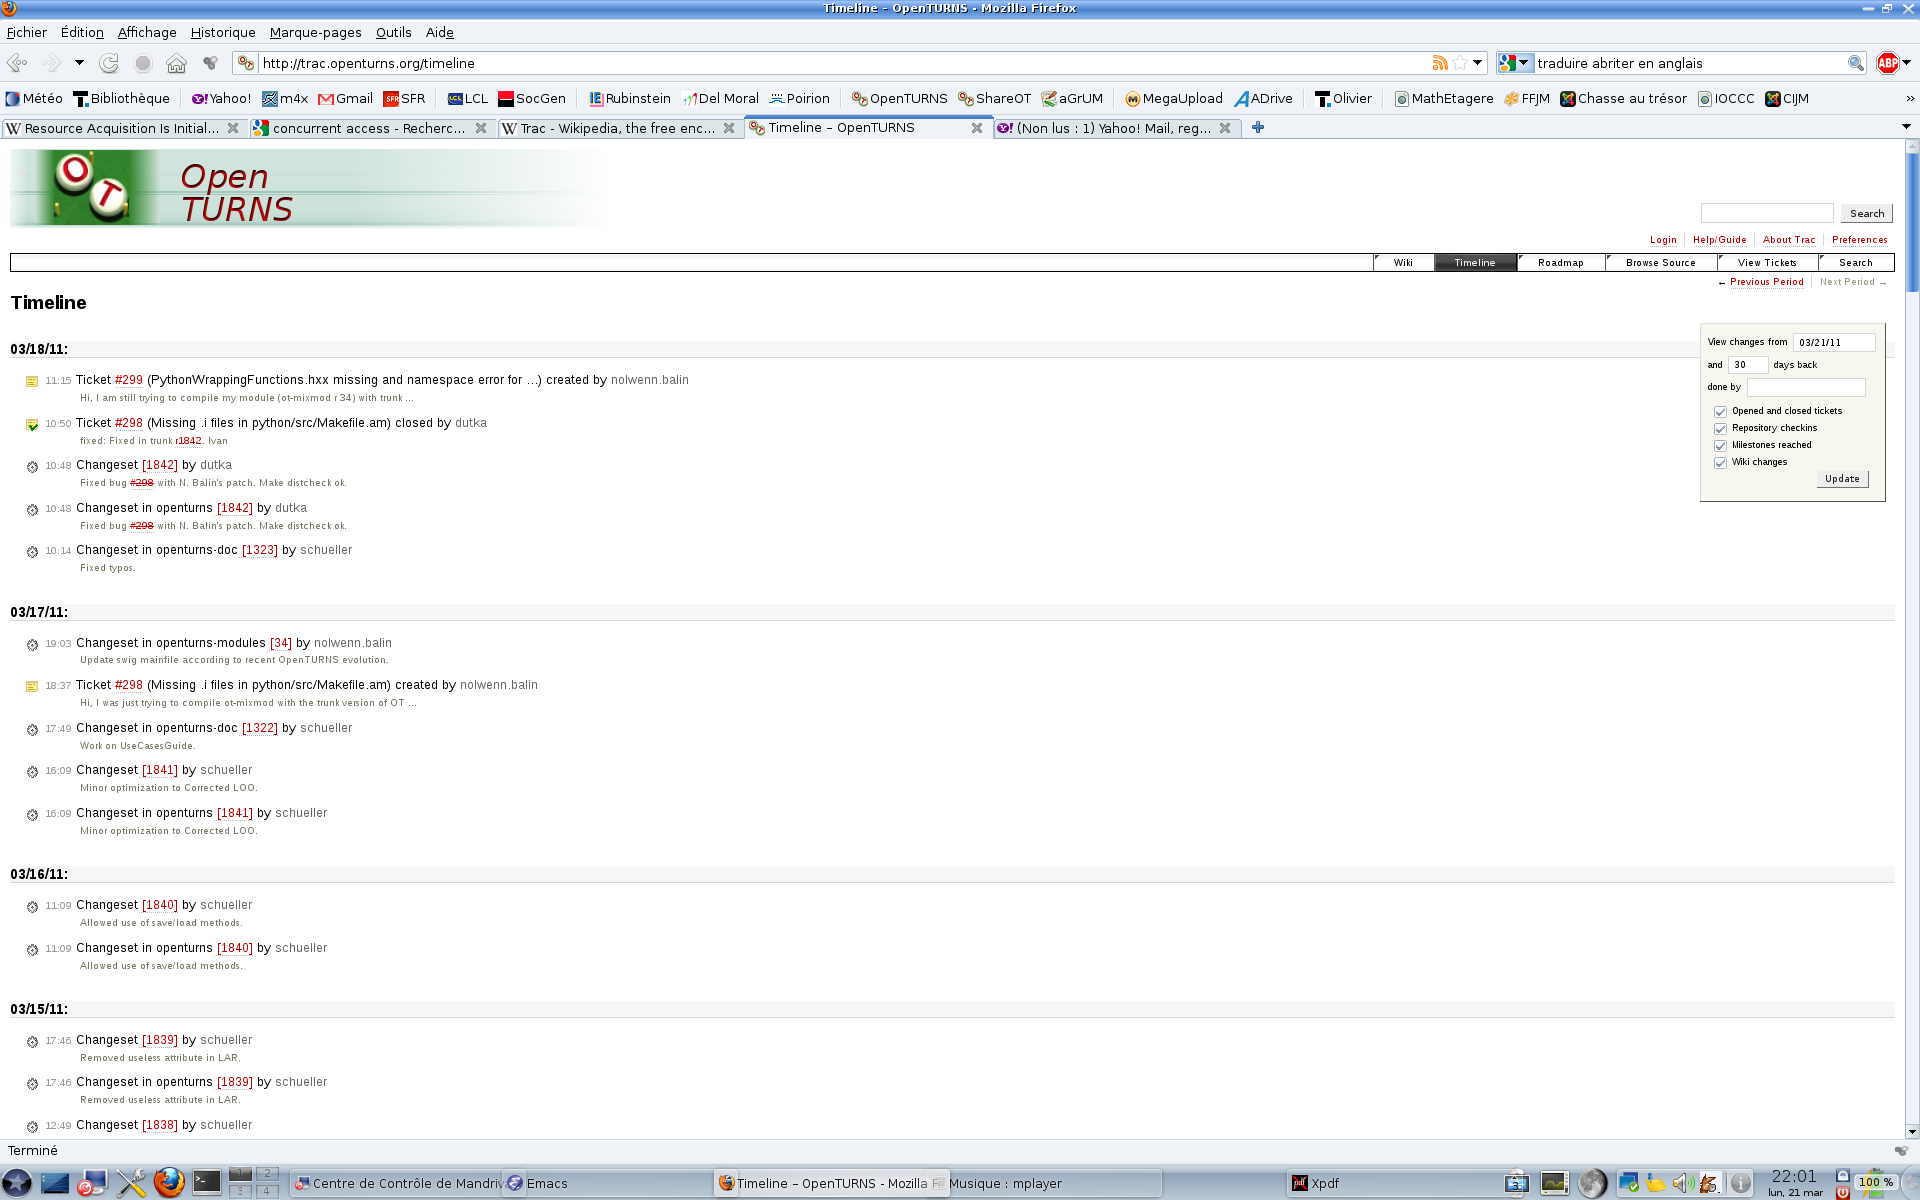
\includegraphics{Timeline.png}}
\end{frame}
%%%%%%%%%%%%%%%%%%%%%%%%%%%%%%%%%% 
% The development infrastructure %
%%%%%%%%%%%%%%%%%%%%%%%%%%%%%%%%%% 
\begin{frame}
  \frametitle{Trac interface: the source navigator}
  \centering \resizebox{!}{7cm}{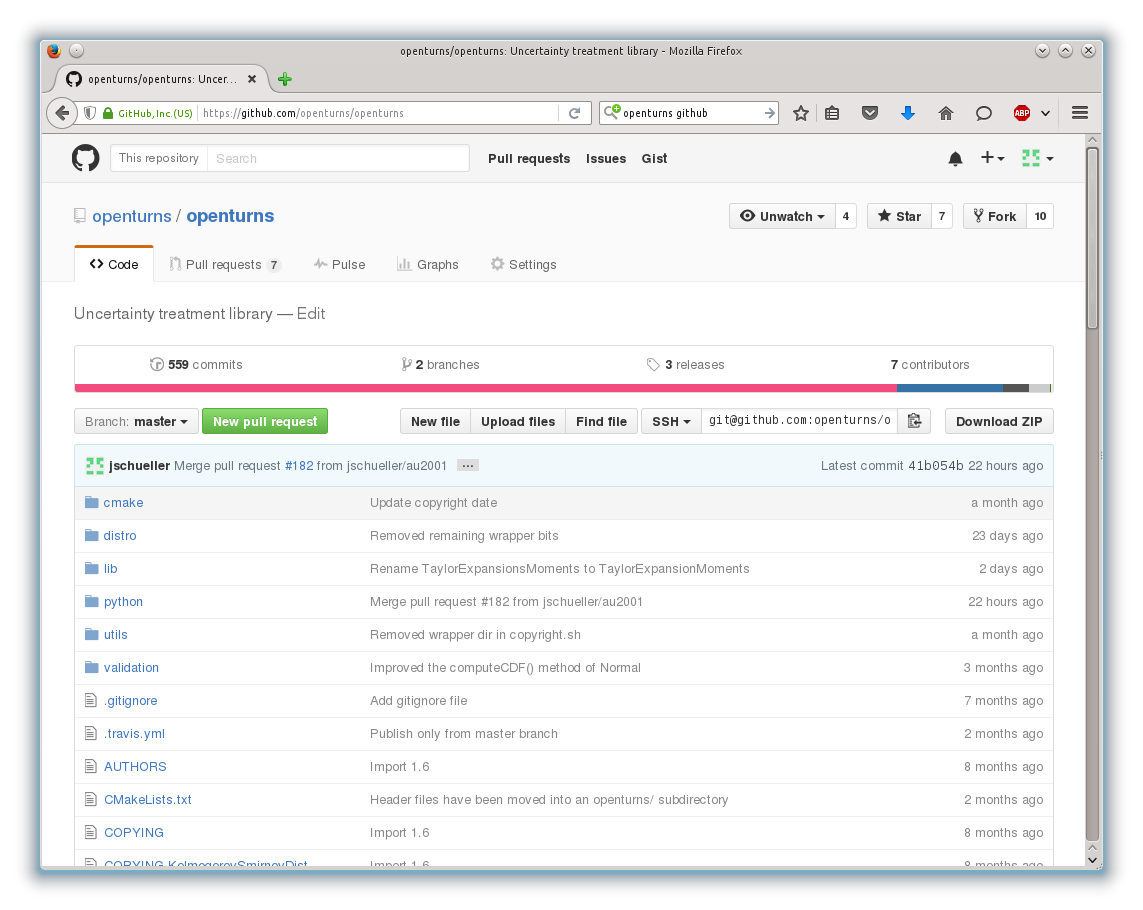
\includegraphics{BrowseSource.png}}
\end{frame}
%%%%%%%%%%%%%%%%%%%%%%%%%%%%%%%%%% 
% The development infrastructure %
%%%%%%%%%%%%%%%%%%%%%%%%%%%%%%%%%% 
\begin{frame}
  \frametitle{Trac interface: the bug tracking (1/2)}
  \centering \resizebox{!}{7cm}{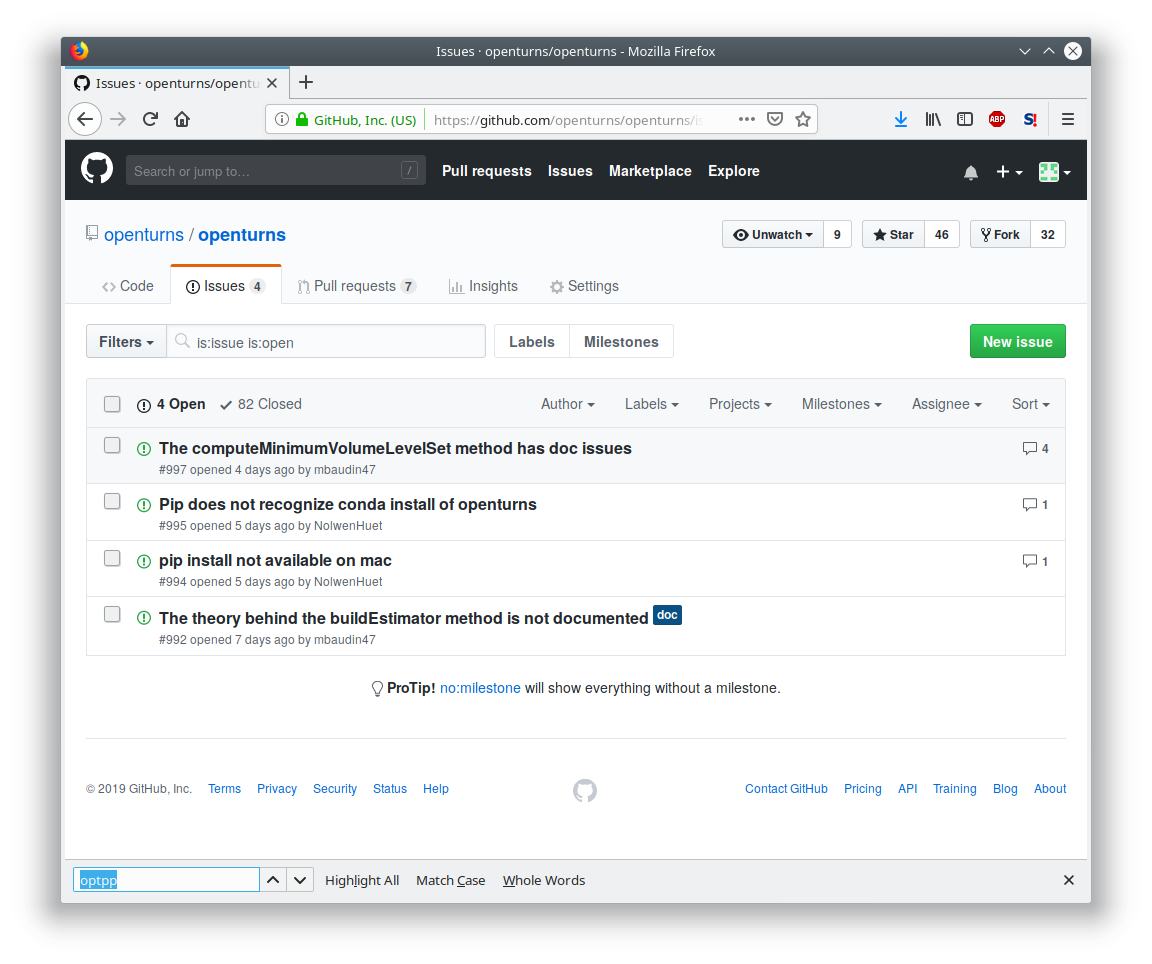
\includegraphics{Tickets1.png}}
\end{frame}
%%%%%%%%%%%%%%%%%%%%%%%%%%%%%%%%%% 
% The development infrastructure %
%%%%%%%%%%%%%%%%%%%%%%%%%%%%%%%%%% 
\begin{frame}
  \frametitle{Trac interface: the bug tracking (2/2)}
  \centering \resizebox{!}{7cm}{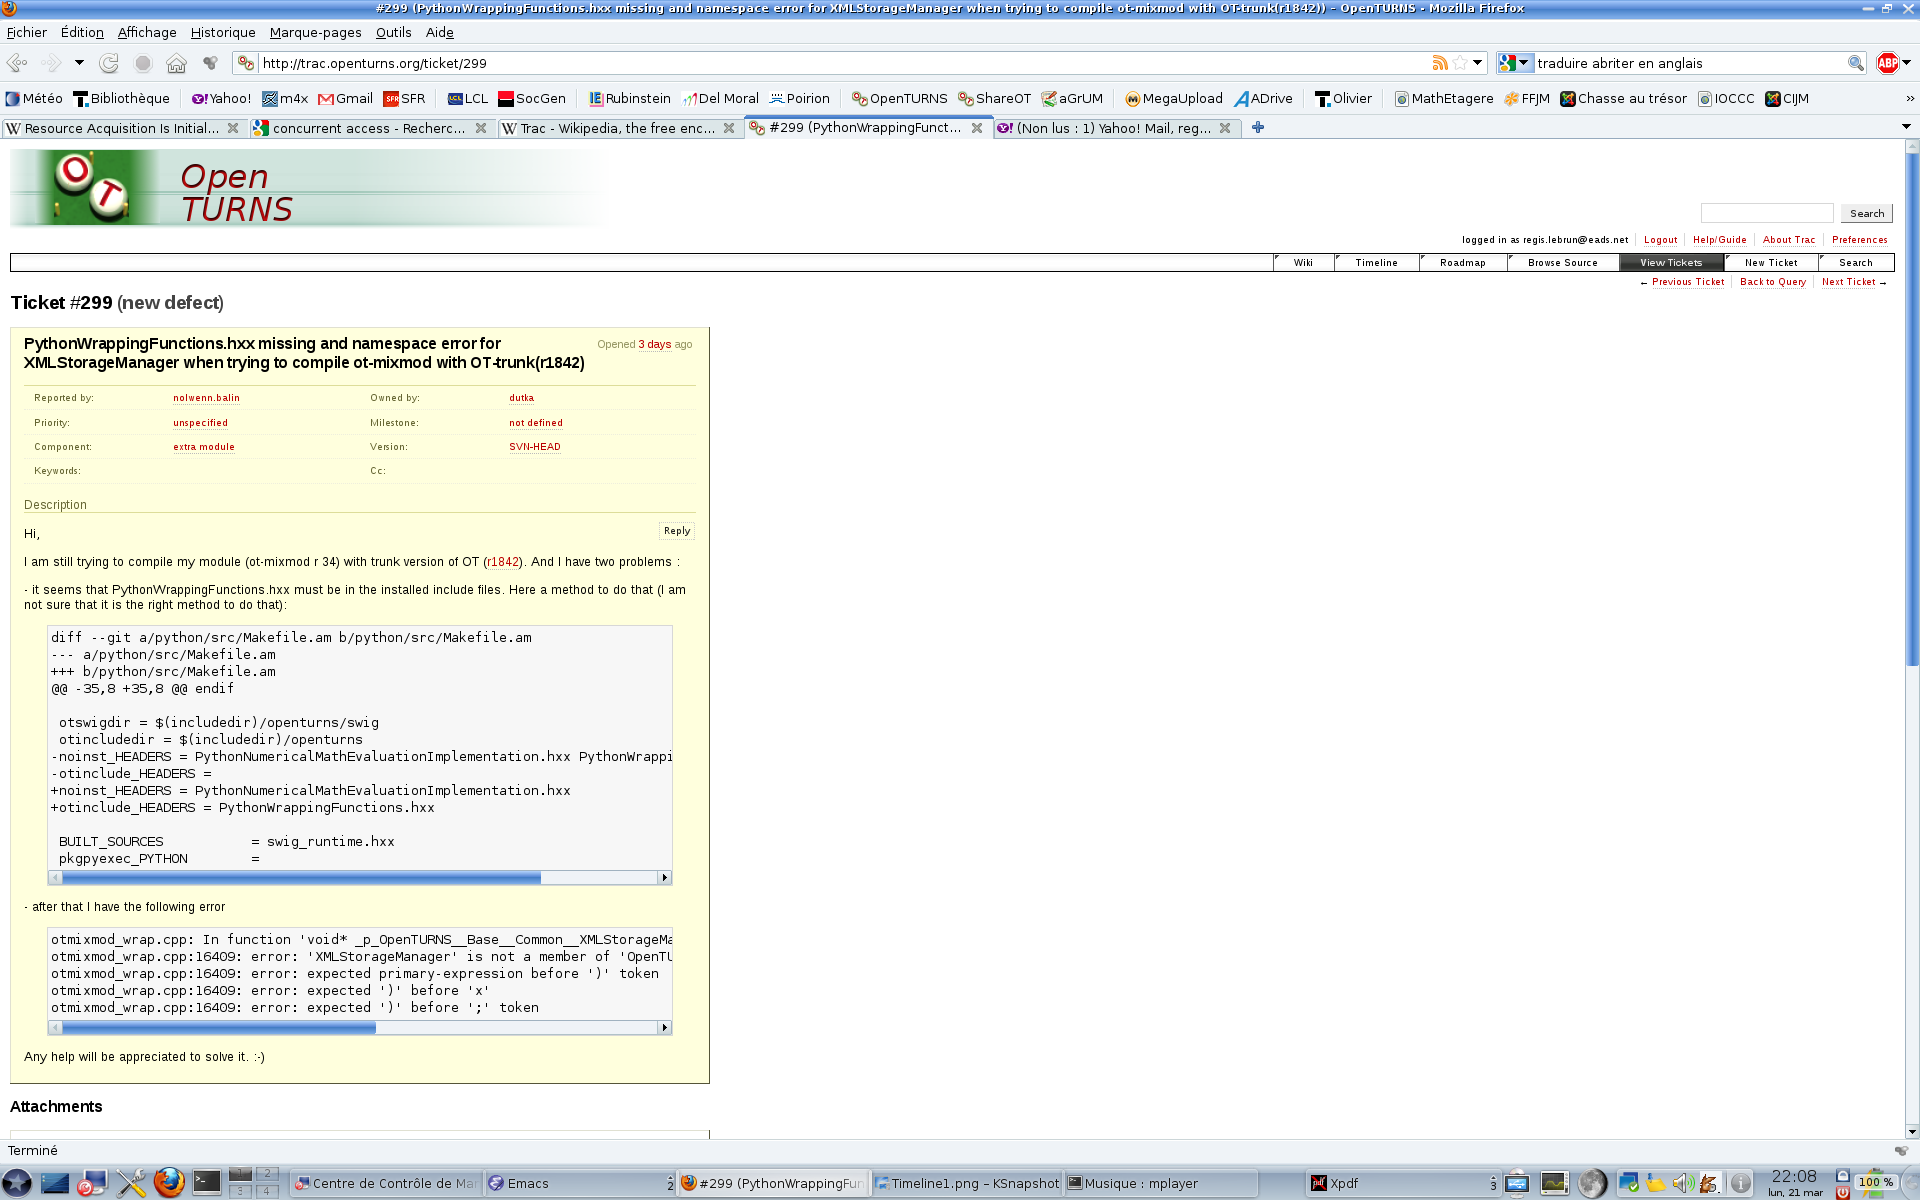
\includegraphics{Tickets2.png}}
\end{frame}
%%%%%%%%%%%%%%%%%%%%%%%%%%%%%%%%%% 
% The development infrastructure %
%%%%%%%%%%%%%%%%%%%%%%%%%%%%%%%%%% 
\section[Conclusion]{Conclusion}
\begin{frame}
  \Large
  \frametitle{Conclusion}
  \begin{itemize}
  \item A quite mature project: 6 full years of development
  \item A structured (rigid ;-)?) development process
  \item A working infrastructure to help the developer in his/her hard job!
  \end{itemize}
\end{frame}
\end{document}

